% Discuss the DOE project and how it is relevant

\chapter{Smart Grid and Smart Meters}
\label{chapter:doe}

\section{Overview}
There has been a move recently towards the design and implementation of what is called a "smart grid." A smart
grid is an electrical power grid which can gather information about the meters, houses, and consumers of
electricity that are attached to it.

By gathering information from a smart grid, a power company can more efficiently manage its production and delivery
of electricity, thus reducing cost. Not only does the smart grid help the power company, but by providing analytics to
its customers, customers can adjust their consumption habits to lower their bills as well. With the increasing cost of
fossil fuels and the increasing energy consumption of today's consumer, reducing wasted electricity will be very useful.

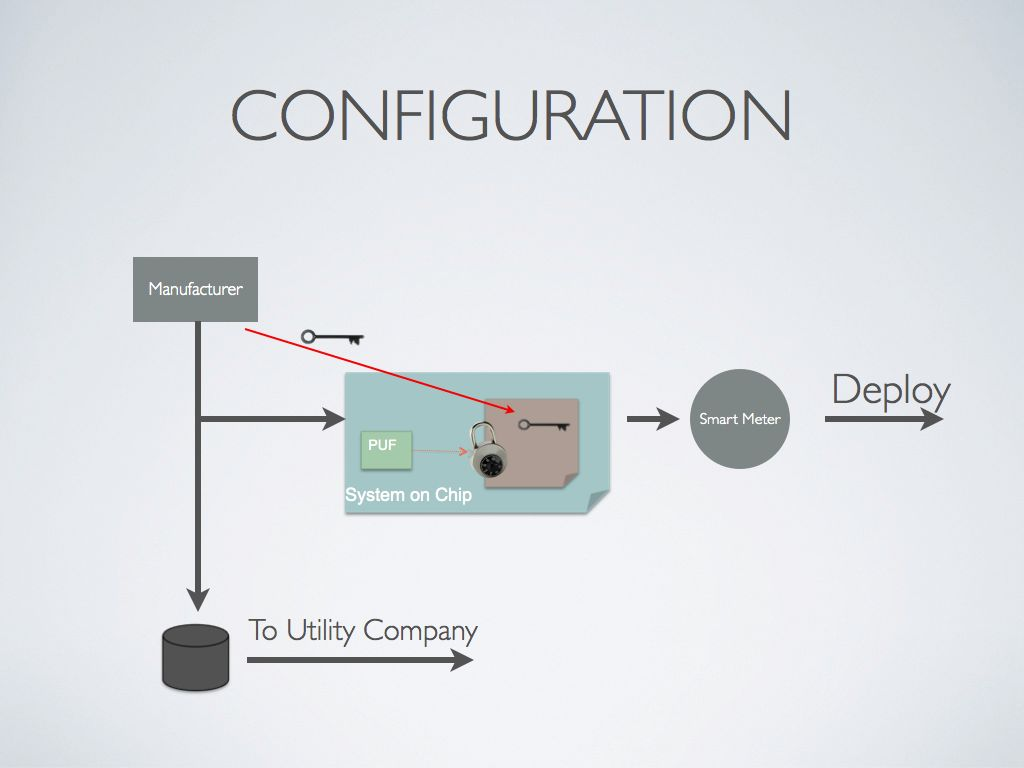
\includegraphics[width=400px]{images/doe_007.jpg}

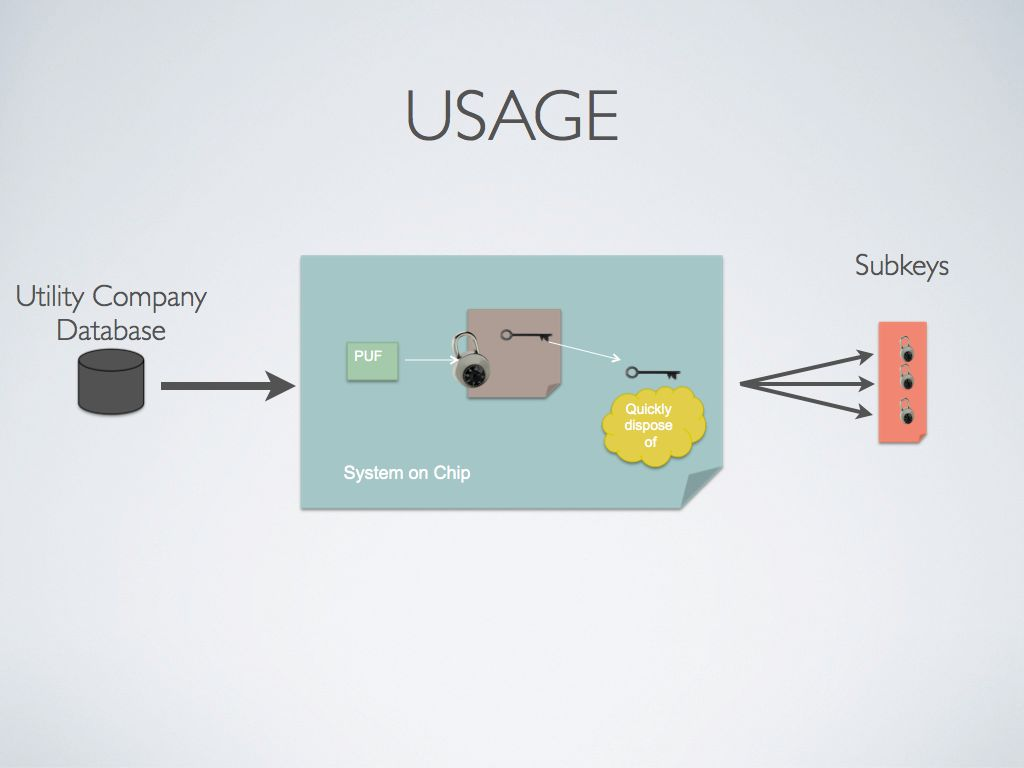
\includegraphics[width=400px]{images/doe_008.jpg}

\section{Implemenation}

\subsection{Limitations}

\section{Future Work}